
\chapter{Introduction}\label{chapter:Introduction}
\renewcommand{\thepage}{\arabic{page}}
\setcounter{page}{1}
\section{Challenges in Power Systems}
One of the key components of the global goal, Net Zero by 2050, is to decarbonize energy systems, which includes increasing renewable energy use and enhancing energy efficiency (\cite{bouckaert2021net}). However, the rising penetration of intermittent renewable energy has significantly strained the grid, making its operation increasingly challenging over the past decades (\cite{shah2015review, impram2020challenges}). Additionally, extreme weather events driven by climate change add further uncertainty to power generation and increase the risk of cascading failures in power grids (\cite{bhusal2020power, xu2024resilience}). The \gls{IEA} affirms that the global energy crisis lies in addressing security issues while accelerating energy transition (\cite{world2023outlook}). Hence, addressing volatile power generation plays a rudimental role in power system.\\
Issues in power balance come from not only the power supply but also power demand. The \gls{IEA} forecasts the energy demand to grow by an average of 3.4\% annually through 2026  (\cite{electricity2024analysis}). As shown in Figure \ref{fig:DemandRegional}, the annual global electricity demand is expected to reach 30700 TWh. As demand grows, the strain on the grid intensifies, potentially leading to overloading of infrastructures and high frequency of peak loads and influencing the grid stability.\\
\begin{figure}[h!]
\begin{center}
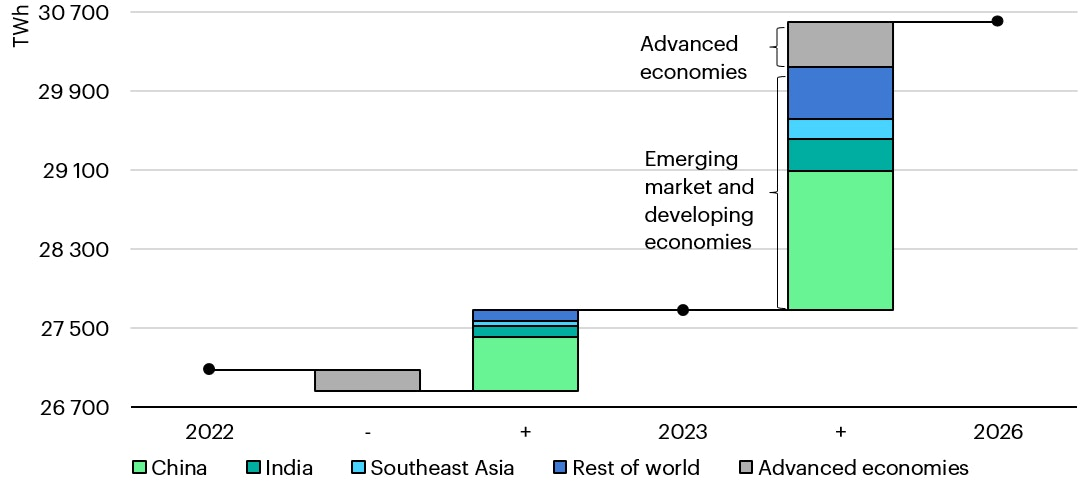
\includegraphics[width=0.9\textwidth]{LaTeX_Vorlagen_Studienarbeiten/images/Global Energy Demand 2022-2026 by region.jpeg}
\caption{Electricity Demand by Region from 2022 to 2026 (\cite{electricity2024analysis})}
\label{fig:DemandRegional}
\end{center}
\end{figure}

\section{Impact of \gls{EV} on Grid Operation}
According to \gls{IEA}, transportation accounts for more than one third of $\text{CO}_{2}$ emissions from end-use sectors. \gls{EV} has become one of the main options for low carbon-intensive transportation, resulting in rising electricity demand as shown in Figure \ref{fig:EV_Demand} (\cite{ev2024outlook}). Even though the electricity demand from \gls{EV} accounts for less than 1\% in 2023, which is relatively low in comparison to other end-use sections, the increasing penetration still poses high stress on the distribution grid. \cite{hilshey2012estimating} estimate the impact of \gls{EV} charging on transformer aging. \cite{wang2021grid} raised the concern of power quality problem resulting from \gls{EV} fast charging points. \cite{wangsness2021impact} confirm uncoordinated \gls{EV} charging can cause higher grid cost. 
\begin{figure}[h!]
\begin{center}
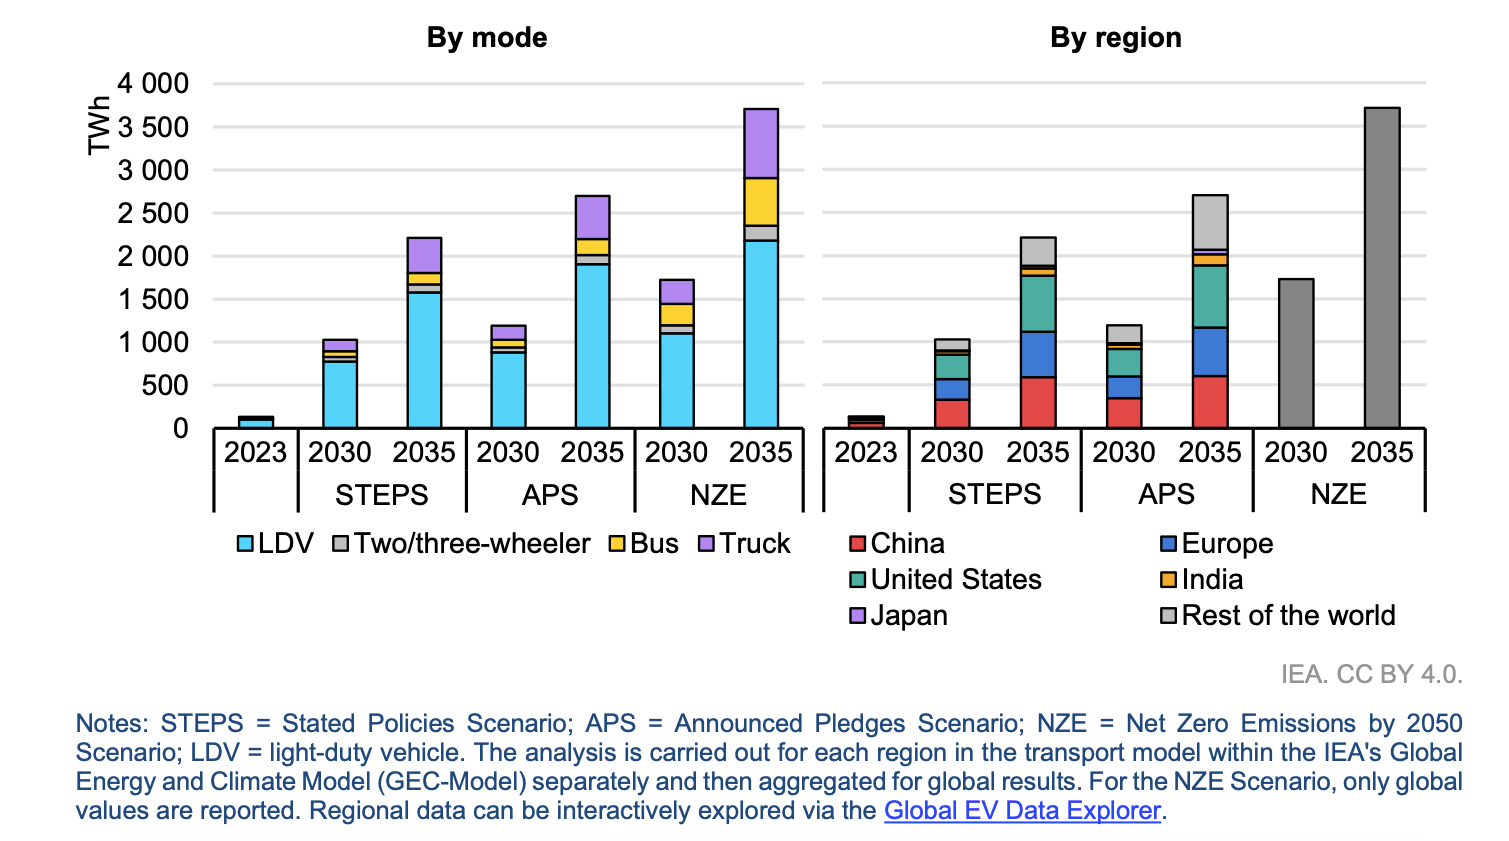
\includegraphics[width=0.9\textwidth]{LaTeX_Vorlagen_Studienarbeiten/images/EV Electricity Demand.png}
\caption{\gls{EV} Electricity Demand by Mode and by Region from 2023 to 2035 (\cite{ev2024outlook})}
\label{fig:EV_Demand}
\end{center}
\end{figure}
Thus, the \gls{DSO}, who is responsible for providing network services for the connection of electricity end-users and distributed generation must consider \gls{EV} charging when dispatching (\cite{eudirective2009}). Many \gls{DSO}s, such as Stadtwerke München, E.ON, and Enel, are currently extending their business in \gls{EV} charging and exploring initiatives to serve as \gls{EV} aggregators. This allows \gls{DSO}s to adapt charging activities in the \gls{EV} charging stations to grid operation. Moreover, with the help of \gls{V2G} technology, it is possible for \gls{DSO}s to use \gls{EV} batteries as a means of demand response. Therefore, it is crucial for \gls{DSO}s to consider \gls{EV} charging behavior when deciding on a power system schedule.%, which can be formulated as an \gls{EV}-aware \gls{OPF} problem.

\section{Optimal Power Flow}
To address instability and facilitate energy transition, \gls{BESS} are often used as a buffer mechanism. However, their high cost and maintenance requirements drive the search for alternatives (\cite{bessa2019handling,islam2019mitigating}). Among all, \gls{OPF} has been the predominant method for addressing both security and economic issues simultaneously in support of power system operation and control.\\
\gls{OPF} is a fundamental problem in power systems optimization, is first introduced by \cite{carpentier1962contribution}. It aims to determine the optimal settings for control variables such as generator output, transformer tap settings, and switching of shunt devices in order to minimize the overall operating cost while satisfying various operational constraints such as power balance, voltage limits, and equipment constraints. \gls{OPF}, typically representing a snapshot of the power system operation, is suitable for short-term operational planning and real-time applications requiring rapid decisions.\\
With the introduction of \gls{BESS} and \gls{EV}, \gls{BESS}- or \gls{EV}-aware \gls{OPF} (also called \gls{MOPF} (\cite{Kayacik2021}))  has become popular. It extends the optimization horizon beyond a single time period to consider the dynamic behavior of the power system over multiple time intervals. It accounts for the time-varying nature of electricity demand, renewable energy generation, and the scheduling of energy resources over a longer planning horizon.\\
\gls{OPF} problem is characterized by several significant challenges, beginning with the inherent non-linearity of the power flow equations that describe the relationships between generation, load, and network parameters (\cite{carpentier1962contribution}). These equations are both nonlinear and non-convex, making the \gls{OPF} problem complex and difficult to solve, particularly when ensuring voltage stability across the network (\cite{mei2008study, yang2017novel}). The non-convex nature that lies in the \gls{OPF} problem can potentially lead to non-convergence in solving algorithms (\cite{avriel2020nonlinear}).\\
Another major challenge is the computational complexity associated with solving \gls{OPF} for large-scale power systems (\cite{yang2016large}). Modern power grids encompass thousands of buses, generators, and transmission lines, demanding substantial computational resources to find optimal solutions, especially in real-time scenarios. \\
Additionally, the increasing integration of renewable energy sources and \gls{EV}s introduces significant uncertainty and variability into the \gls{OPF} problem (\cite{jabr2014robust}). The intermittent nature of renewable energy generation and the fast-charging demands of \gls{EV}s necessitate the use of robust or stochastic optimization techniques to manage these uncertainties (\cite{wang2021grid}). Combined with potential errors in load forecasting, these factors further complicate the search for robust and efficient \gls{OPF} solutions. Ensuring this robustness often requires conservative approximations, which can lead to suboptimal results, balancing the need for reliability with efficiency (\cite{ding2016adjustable}).
%A further challenge in the \gls{OPF} problem is ensuring both the convergence of the optimization algorithms and the robustness of the solutions. Given the complexity and scale of power systems, especially with their nonlinear and non-convex characteristics, achieving global convergence to an optimal solution is often difficult. Algorithms may struggle to find the best solution, particularly in large-scale or highly constrained problems. Moreover, the OPF solution must be robust to uncertainties in system parameters, such as transmission line impedances, generator characteristics, and load forecasts. Ensuring this robustness often requires conservative approximations, which can lead to suboptimal results, balancing the need for reliability with efficiency.


%\renewcommand{\thepage}{\arabic{page}}
%\setcounter{page}{1}
